\chapter{Contexte}

%%%
\section{Vers une robotique collaborative}
%%%

\subsection{L'émergence de la robotique collaborative et ses enjeux}

\subsubsection{Génèse de la robotique}

\subsubsection{Vers une collaboration humain-robot}

\subsection{Vers quels types de collaboration ?}

\subsubsection{Les environnements collaboratifs}

\subsubsection{Les modalités de collaboration}

\subsubsection{Les interactions haptique}

\subsection{Les contrôles robotiques lors d'interactions physiques}

%%%
\section{Modéliser le comportement humain}
%%%

\subsection{Les sciences du mouvement humain}

\subsection{Modéliser le comportement humain en interaction physique grâce à l'impédance}

\subsubsection{Définition}

%Le \textit{Random House Kernerman Webster's College Dictionary} définit l'impédance mécanique comme, le rapport entre une \emph{force} exercée sur un système physique soumis à un \emph{mouvement} harmonique, et la \emph{vitesse} des particules du-dit système\footnote{"\textit{The ratio of the force on a system undergoing harmonic motion to the velocity of the particles in the system.}"}. De manière plus générale, \cite{hogan_impedance_1985} explique que les systèmes physiques peuvent soit être définis en impédance, c'est à dire qu'ils acceptent en entrée un flux et fournissent en sortie un effort, soit en admittance, l'inverse de l'impédance. Ce concept d'abord établi pour l'électricité, est donc élargi à tous les systèmes physiques, ainsi, l'impédance mécanique se précise (\cref{mec_impedance}) comme une \emph{résistance à un mouvement}.

L'\emph{impédance} $H$, peut se définir pour un système, comme le rapport d'un \emph{potentiel} extensif $E$ sur un \emph{flux} intensif $\phi$. Dit autrement, il s'agit de la capacité d'un système dynamique, d'opposer une force dont l'intensité est proportionnelle à une quantité caractéristique variable dans le temps, lorsqu'il est soumis à un flux de particules en mouvements.

\begin{equation}
	E(t) = H(t)\phi(t)
	\label{eq_impedance_gen}
\end{equation}

L'inverse de l'impédance, parfois abusivement désigné par le même mot, se nomme l'admittance, comme explicité sur la \cref{fig_impedance_physique}.

\begin{figure}[h]
	\centering
	\resizebox{\textwidth}{!}{	
	\begin{tikzpicture}
	\node[rectangle, draw, align=center, minimum width=3.5cm, minimum height=1.75cm, line width=1.2, font=\large] (impedance) at (0,0) {\emph{Impédance}};
	\node[rectangle, draw, align=center, minimum width=3.5cm, minimum height=1.75cm, line width=1.2, font=\large] (admittance) at ($(impedance) + (6.5, 0)$) {\emph{Admittance}};
	\draw[-{Latex[length=3mm]}, line width=1.2] (impedance.east) -- (admittance.west)
	node[midway, above] {\phantom{p}potentiel\phantom{p}};
	\draw[{Latex[length=3mm]}-, line width=1.2] (impedance.west) -- +(-2.8,0)
	node[midway, above] {\phantom{p}flux\phantom{p}};		
	\draw[-{Latex[length=3mm]}, line width=1.2] (admittance.east) -- +(2.8,0)
	node[midway, above] {\phantom{p}flux\phantom{p}};
	\end{tikzpicture}
	}	
	\caption{Systèmes physiques} % Figure caption
	\label{fig_impedance_physique} % Label for referencing
\end{figure}

Le concept d'impédance a été introduit dans un premier temps à la fin du XIXème siècle \cite{noauthor_impedance_nodate}, comme une généralisation de la loi d'Ohm au courant alternatif. Ainsi, l'impédance électrique se définit comme la résistance $Z$ d'un circuit électrique à un flux de courant $i$ en lui opposant une tension électrique $U$. D'où le nom proposé par O. Heaviside de "\textit{impedance}", dérivé du verbe anglais "\textit{impede}" qui peut se traduire par retenir.

\begin{equation}
	U(t) = Z i(t)
	\label{eq_impedance_elec}
\end{equation}

Le concept d'impédance s'est ensuite étendu à d'autres grandeurs physiques comme l'acoustique, la thermique et la \emph{mécanique}. L'impédance mécanique $H$ décrit ainsi la quantité de force $F$ qu'oppose un système physique lorsqu'il est soumis à une vitesse $v$. L'impédance mécanique peut donc être considérée comme une résistance à un mouvement, et à l'inverse, l'admittance mécanique comme la maniabilité d'un système physique, c'est à dire sa capacité à se déplacer lorsqu'une force lui est appliqué.

\begin{equation}
	F(t) = H v(t)
	\label{eq_impedance_mec}
\end{equation}

Ainsi, par analogie avec l'électricité, dans le cas restreint des systèmes linéaires unidimensionnels, il existe trois éléments passifs pour l'impédance mécanique, qui sont la \emph{masse}, la \emph{raideur} et l'\emph{amortissement} que l'on peut rapprocher respectivement à l'inductance, la capacité et la résistance ; et deux éléments actifs, la force et la vitesse qui peuvent être mis en parallèle à la tension et au courant. 

Comme c'est le cas pour l'électricité, il est possible d'exprimer l'impédance mécanique dans un plan complexe \cite{hondori_method_2009}, mais cette représentation est assez marginale lorsqu'on parle de l'impédance mécanique chez l'Homme.\\

L'impédance mécanique permet donc de modéliser les relations entre les forces et les mouvements qui sont appliqués sur un système. On trouve ainsi des modèles dynamiques uniarticulaires de membres du corps humain, par exemple du coude \cite{de_rugy_actively_2003, avrin_particle_2016}, comme montré sur \cref{eq_impedance_artic_mvt_derugy}. Dans ces cas, le mouvement du bras $\theta$ est obtenu à partir des couples appliqués par les muscles agonistes $T_i$ (eg. biceps) et antagonistes $T_j$ (eg. triceps), dans le cas de mouvements rythmiques. On retrouve ainsi les éléments caractéristiques de la mécanique linéaire, avec la raideur $k$, l'amortissement $\gamma$ et l'inertie $I$.

Les couples musculaires sont alors considérés comme proportionnel à une commande neurale, générée à l'aide d'un oscillateur non linéaire bio-inspiré, proposé par \cite{matsuoka_sustained_1985}. C'est l'appoche de computationnelle de contrôle en force telle qu'expliquée par \cite{danion_we_2011}.

\begin{equation}
	I\ddot{\theta} + \gamma\dot{\theta} + k\theta = T_i + T_j
\label{eq_impedance_artic_mvt_derugy}
\end{equation}

L'impédance permet aussi de décrire les interactions physiques entre plusieurs systèmes dynamiques en contact. On peut alors décorréler la génération du mouvement, du comportement de rejet des perturbations.

\subsubsection{Les types de modélisation}

Si l'on considère l'articulation d'un membre, une même trajectoire peut être décrite avec des cocontractions variées - \textit{c'est à dire aussi bien la contraction des muscles générant le mouvement (agoniste), que deux ceux s'y opposant (antagoniste)} -, que ce soit dans le cas de trajectoire statique et donc isométrique \cite{dolan_dynamic_1993, d_j_newham_knee_2001}, ou en mouvement \cite{yamazaki_reciprocal_1994, milner_damping_1998, gribble_role_2003}. 

Ainsi, \cite{gribble_role_2003} ont montré que les cocontractions du membre supérieur augmentaient lorsque la précision requise pour une tâche de pointage augmentait. Des mesures de l'activité musculaire étaient effectuées à l'aide de capteur EMG pendant la tâche, ainsi que sur une durée de \SI{200}{\milli\second} après l'arrêt du mouvement. Lorsque la taille de la cible diminuait, les cocontractions augmentaient et les erreurs de mouvement diminuaient. Ces résultats suggèrent selon les auteurs, que de système nerveux central peut adapter les cocontractions pour améliorer la précision d'un mouvement, et aussi son rejet des perturbations externes.

En effet comme le témoignent plusieurs travaux, les cocontractions musculaires ont notamment pour effet d'augmenter la robustesse en assurant des marges de stabilité plus importante \cite{granata_costbenefit_2000, milner_adaptation_2002, gribble_role_2003, darainy_muscle_2008}. [Ajouter du texte sur la possibilité d'assimiler les cocontractions a un comportement en raideur...]

\cite{milner_adaptation_2002} ont conduit une expérience sur l'articulation du poignet d'une dizaine de participants à l'aide d'un manipulandum. Pendant des mouvements rapides (\SI{3.14}{\radian\per\second}) et lents (\SI{0.57}{\radian\per\second}) de \ang{20}, avec des charges variables, dépendantes de la position - \textit{raideur négative} -, de la vitesse - \textit{amortissement négatif} - et des vibrations à \SI{5.5}{\hertz} et \SI{10}{\hertz}, les participants devaient réaliser une tâche de pointage uni-articulaire. Des mesures EMGs étaient enregistrées à partir de \SI{250}{\milli\second} avant et jusqu'à \SI{1500}{\milli\second} après le déclenchement du mouvement, sur six muscles responsable des flexions et extensions du poignet. Le critère de stabilité était évalué par rapport au décrément des oscillations en position une fois la cible atteinte. Ainsi, après avoir demandé aux participants de réduire au plus vite ces oscillations, si des mouvements en dehors d'une cible de \ang{3} étaient observés après \SI{800}{\milli\second}, alors le mouvement était considéré non conforme au critère de stabilité. Les résultats de l'étude indiquent que les cocontrations étaient impliquées à différent degré pour stabiliser le poignet en présence d'environnement déstabilisant.

Des résultats similaires sont observés pour d'autres parties du corps par \cite{cholewicki_stabilizing_1997, granata_costbenefit_2000} concernant les muscles du tronc, par \cite{hogan_adaptive_1984, de_serres_wrist_1991, burdet_central_2001} pour les muscles des membres supérieurs et par \cite{hirokawa_muscular_1991, finley_contributions_2012, di_nardo_assessment_2015, kim_center_2018} pour les muscles des membres inférieurs. Ainsi les cocontractions contribuent à améliorer la robustesse d'une articulation lorsqu'elle peut être soumise à des perturbations. Il est toutefois important de souligner qu'il ne s'agit qu'un seul des mécanismes existants permettant d'assurer la stabilité d'un mouvement ou du maintient d'une posture. 

Comme l'expliquent \cite{finley_contributions_2012}, dans le cadre d'une expérience où des participants essaient de stabiliser un modèle simplifié de l'humain à l'aide de mouvements de leur cheville, la raideur générée par les cocontractions seules ne permet pas d'assurer la stabilité. Ainsi pour les auteurs, les propriétés mécaniques intrinsèques de la cheville ne sont pas suffisantes et des modulations actives et donc volontaires des muscles sont nécessaires [contribution des réflexes]. La \cref{fig_experience_finley_2012} reprend le schéma expérimental présenté par les auteurs dans leur publication. %L'objectif de cette expérience étant de se placer dans un cas simplifié du corps humain, où se dernier n'est représenté que par un simple pendule inversé d'une masse de \SI{25}{\percent} de celle de chaque participant et d'une hauteur de \SI{1}{\meter}.

\begin{figure}[h]
	\centering
	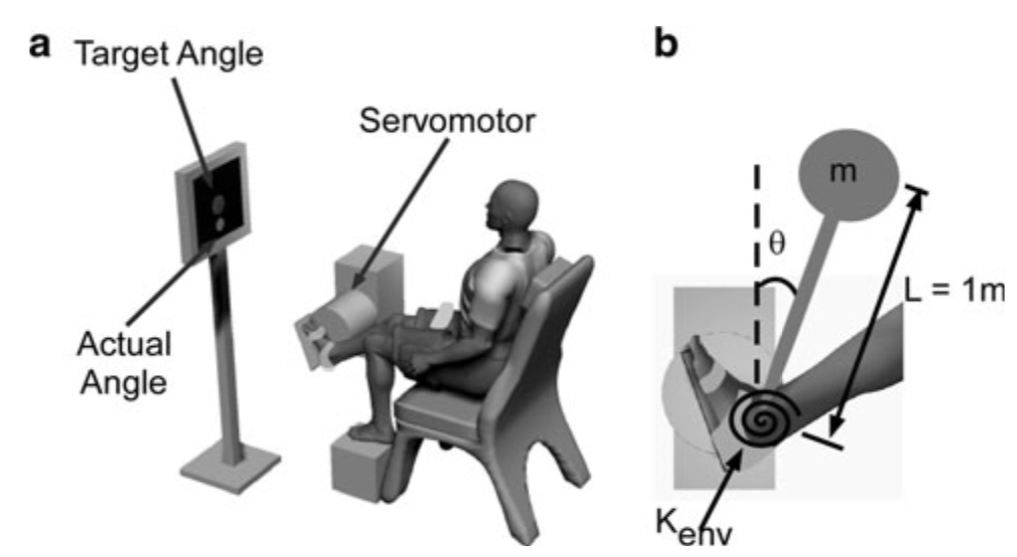
\includegraphics[width=0.9\textwidth]{misc/fig_experience_finley_2012}
	\caption{Experimental setup for study of ankle control. a) Subjects wereseated with their foot attached to a servomotor via a rigid foot plate.Individuals used visual feedback of the foot plate angle to maintainthe target ankle position. b) Subjects controlled an unstable haptic loadwhich  behaved  like  an  inverted  pendulum  supported  by  a  torsionalspring of stiffnessKenv. The simulated pendulum had a mass equal to \SI{25}{\percent} of the subject’s mass and a height of \SI{1}{\meter}}
	\label{fig_experience_finley_2012}
\end{figure}

[la représentation mécanique du comportement en impédance du corps humain ne se limite pas à la raideur des cocontractions, mais peut intérgrer des comportements réflexes...]

%%%
\section{Problématiques et contributions}
%%%
